% =============================================================================
% MoveLink - Labor-/Projektbericht
% Software-Architekturen Labor, SS 2026
% Hochschule Karlsruhe (HKA)
% =============================================================================
\documentclass[11pt, a4paper]{article}

% --- Pakete ---
\usepackage[ngerman]{babel}
\usepackage[utf8]{inputenc}
\usepackage[T1]{fontenc}
\usepackage{lmodern}
\usepackage[left=2.5cm, right=2.5cm, top=2.5cm, bottom=2.5cm]{geometry}
\usepackage{graphicx}
\usepackage{xcolor}
\usepackage{hyperref}
\usepackage{enumitem}
\usepackage{tabularx}
\usepackage{booktabs}
\usepackage{tikz}
\usepackage{float}
\usepackage{fancyhdr}
\usepackage{titlesec}
\usepackage{parskip}
\usepackage{microtype}
\usepackage{mdframed}
\usepackage{tocloft}
\usepackage[document]{ragged2e}
\emergencystretch=2em
\hyphenpenalty=10000
\exhyphenpenalty=10000

% X-Spalten in tabularx global linksbündig (kein Blocksatz in Tabellen)
\renewcommand{\tabularxcolumn}[1]{>{\raggedright\arraybackslash}p{#1}}

% --- Inhaltsverzeichnis Styling ---
% Überkapitel: rot und fett
\renewcommand{\cftsecfont}{\bfseries\color{hkared}}
\renewcommand{\cftsecpagefont}{\bfseries\color{hkared}}
% Unterkapitel: schwarz (hidelinks im TOC nötig damit hyperref nicht überschreibt)
\renewcommand{\cftsubsecfont}{\normalfont\color{black}}
\renewcommand{\cftsubsecpagefont}{\normalfont\color{black}}
% Spacing: gleiches Spacing auf allen Ebenen
\setlength{\cftbeforesecskip}{8pt}
\setlength{\cftbeforesubsecskip}{8pt}
\setlength{\cftbeforesubsubsecskip}{8pt}
% Abstand nach dem Titel "Inhaltsverzeichnis" vor dem ersten Eintrag
\setlength{\cftaftertoctitleskip}{1.2cm}

% --- Farben (HKA Corporate) ---
\definecolor{hkared}{RGB}{198, 42, 18}
\definecolor{hkagray}{RGB}{100, 100, 100}
\definecolor{placeholderbg}{RGB}{255, 248, 220}
\definecolor{placeholderborder}{RGB}{200, 150, 0}

% --- Hyperref Setup ---
\hypersetup{
    colorlinks=true,
    linkcolor=hkared,
    urlcolor=hkared,
    citecolor=hkared
}

% --- Section Styling ---
\titleformat{\section}{\large\bfseries\color{hkared}}{\thesection}{1em}{}
\titleformat{\subsection}{\normalsize\bfseries\color{hkared}}{\thesubsection}{1em}{}
\titleformat{\subsubsection}{\normalsize\bfseries\color{black}}{\thesubsubsection}{1em}{}
\titlespacing*{\section}{0pt}{1.4em}{0.5em}
\titlespacing*{\subsection}{0pt}{0.8em}{0.3em}
\titlespacing*{\subsubsection}{0pt}{0.6em}{0.2em}

% --- Platzhalter-Umgebung ---
\newmdenv[
    backgroundcolor=placeholderbg,
    linecolor=placeholderborder,
    linewidth=1.5pt,
    roundcorner=4pt,
    innertopmargin=8pt,
    innerbottommargin=8pt,
    innerleftmargin=10pt,
    innerrightmargin=10pt,
    skipabove=8pt,
    skipbelow=8pt
]{placeholder}

% --- Header/Footer ---
\pagestyle{fancy}
\fancyhf{}
\fancyhead[L]{\small\color{hkagray}MoveLink -- Projektbericht}
\fancyhead[R]{\small\color{hkagray}SWA Labor SS~2026}
\fancyfoot[C]{\small\color{hkagray}\thepage}
\renewcommand{\headrulewidth}{0.4pt}

% =============================================================================
\begin{document}

% --- Titelseite ---
\begin{titlepage}
    \centering
    
\includegraphics[width=0.35\textwidth]{HKA.jpg}

    {\normalsize\color{hkagray} University of Applied Sciences}\\[0.125cm]
    {\small\color{hkagray} Fakult\"at f\"ur Informatik und Wirtschaftsinformatik}

    \vspace{.5cm}
    {\color{hkared}\rule{\textwidth}{1.5pt}}

    \vspace{1.5cm}
    {\fontsize{24}{30}\selectfont\bfseries\color{hkared} MoveLink}\\[0.6cm]
    {\Large Visualisierung von Echtzeit-Bewegungsdaten}\\[.75cm]
    {\LARGE\bfseries Projektbericht}

    \vspace{.5cm}
    {\large Software-Architekturen Labor}\\[0.3cm]
    {\large Sommersemester 2026}

    \vspace{.5cm}
    {\color{hkared}\rule{0.6\textwidth}{0.5pt}}
    \vspace{1.5cm}

    {\normalsize
    \begin{tabular}{rl}
        \textbf{Betreuer:}  & Prof.~Dr.~rer.~nat.~Sinz \\[0.5cm]
        \textbf{Team:}      & Erlind Sejdiu \\
                             & Luca Sch\"oneberg \\
                             & Devin Uyan \\[0.5cm]
        \textbf{Abgabe:}    & Ende Sommersemester 2026 \\
    \end{tabular}
    }

    \vfill
    {\small\color{hkagray} Version 2.0 -- Stand: \today}
\end{titlepage}

% --- Inhaltsverzeichnis ---
\begingroup
\hypersetup{hidelinks}
\tableofcontents
\endgroup
\thispagestyle{empty}
\newpage
\setcounter{page}{1}

% =============================================================================
\section{Einleitung}
% =============================================================================
\vspace{.5cm}
\subsection{Motivation}
\vspace{.5cm}

Die Qualit\"at der Bewegungsausf\"uhrung ist im Krafttraining oder in der Physiotherapie ein wichtiger Faktor f\"ur den Trainingserfolg. W\"ahrend professionelle Athleten Zugang zu Coaches und Physiotherapeuten haben, trainieren Otto-normal-Sportler ohne objektives Feedback. Fehler in der Technik, beispielsweise ein zu stark gerundeter R\"ucken bei der Kniebeuge, werden dadurch oft \"uber lange Zeit nicht korrigiert und k\"onnen zu Beschwerden f\"uhren.

Zwar können Bewegungsabläufe durch moderne Hardware-Sensoren erfasst werden, jedoch liegen diese Informationen oft nur als unstrukturierte Rohdaten vor, die für den Endanwender kaum interpretierbar sind. Daraus ergibt sich die Herausforderung, die anfallenden Datenströme aus verschiedenen Quellen zentral zusammenzuführen und visuell nutzergerecht aufzubereiten. \vspace{.25cm}

\subsection{Zielsetzung}
Im Rahmen dieses Laborprojekts wird die mobile Applikation \textbf{MoveLink} konzipiert und prototypisch entwickelt. Ziel der Anwendung ist es, als zentrale Schnittstelle zu fungieren, die Trainingsdaten von unterschiedlichen Hardware-Sensoren erfasst, speichert und in einer einheitlichen Benutzeroberfläche verständlich darstellt.

\newpage

% =============================================================================
\section{System Kontext, Use Cases und Anforderungen}
% =============================================================================
\subsection{System Kontext}

\begin{figure}[h!]
    \centering
    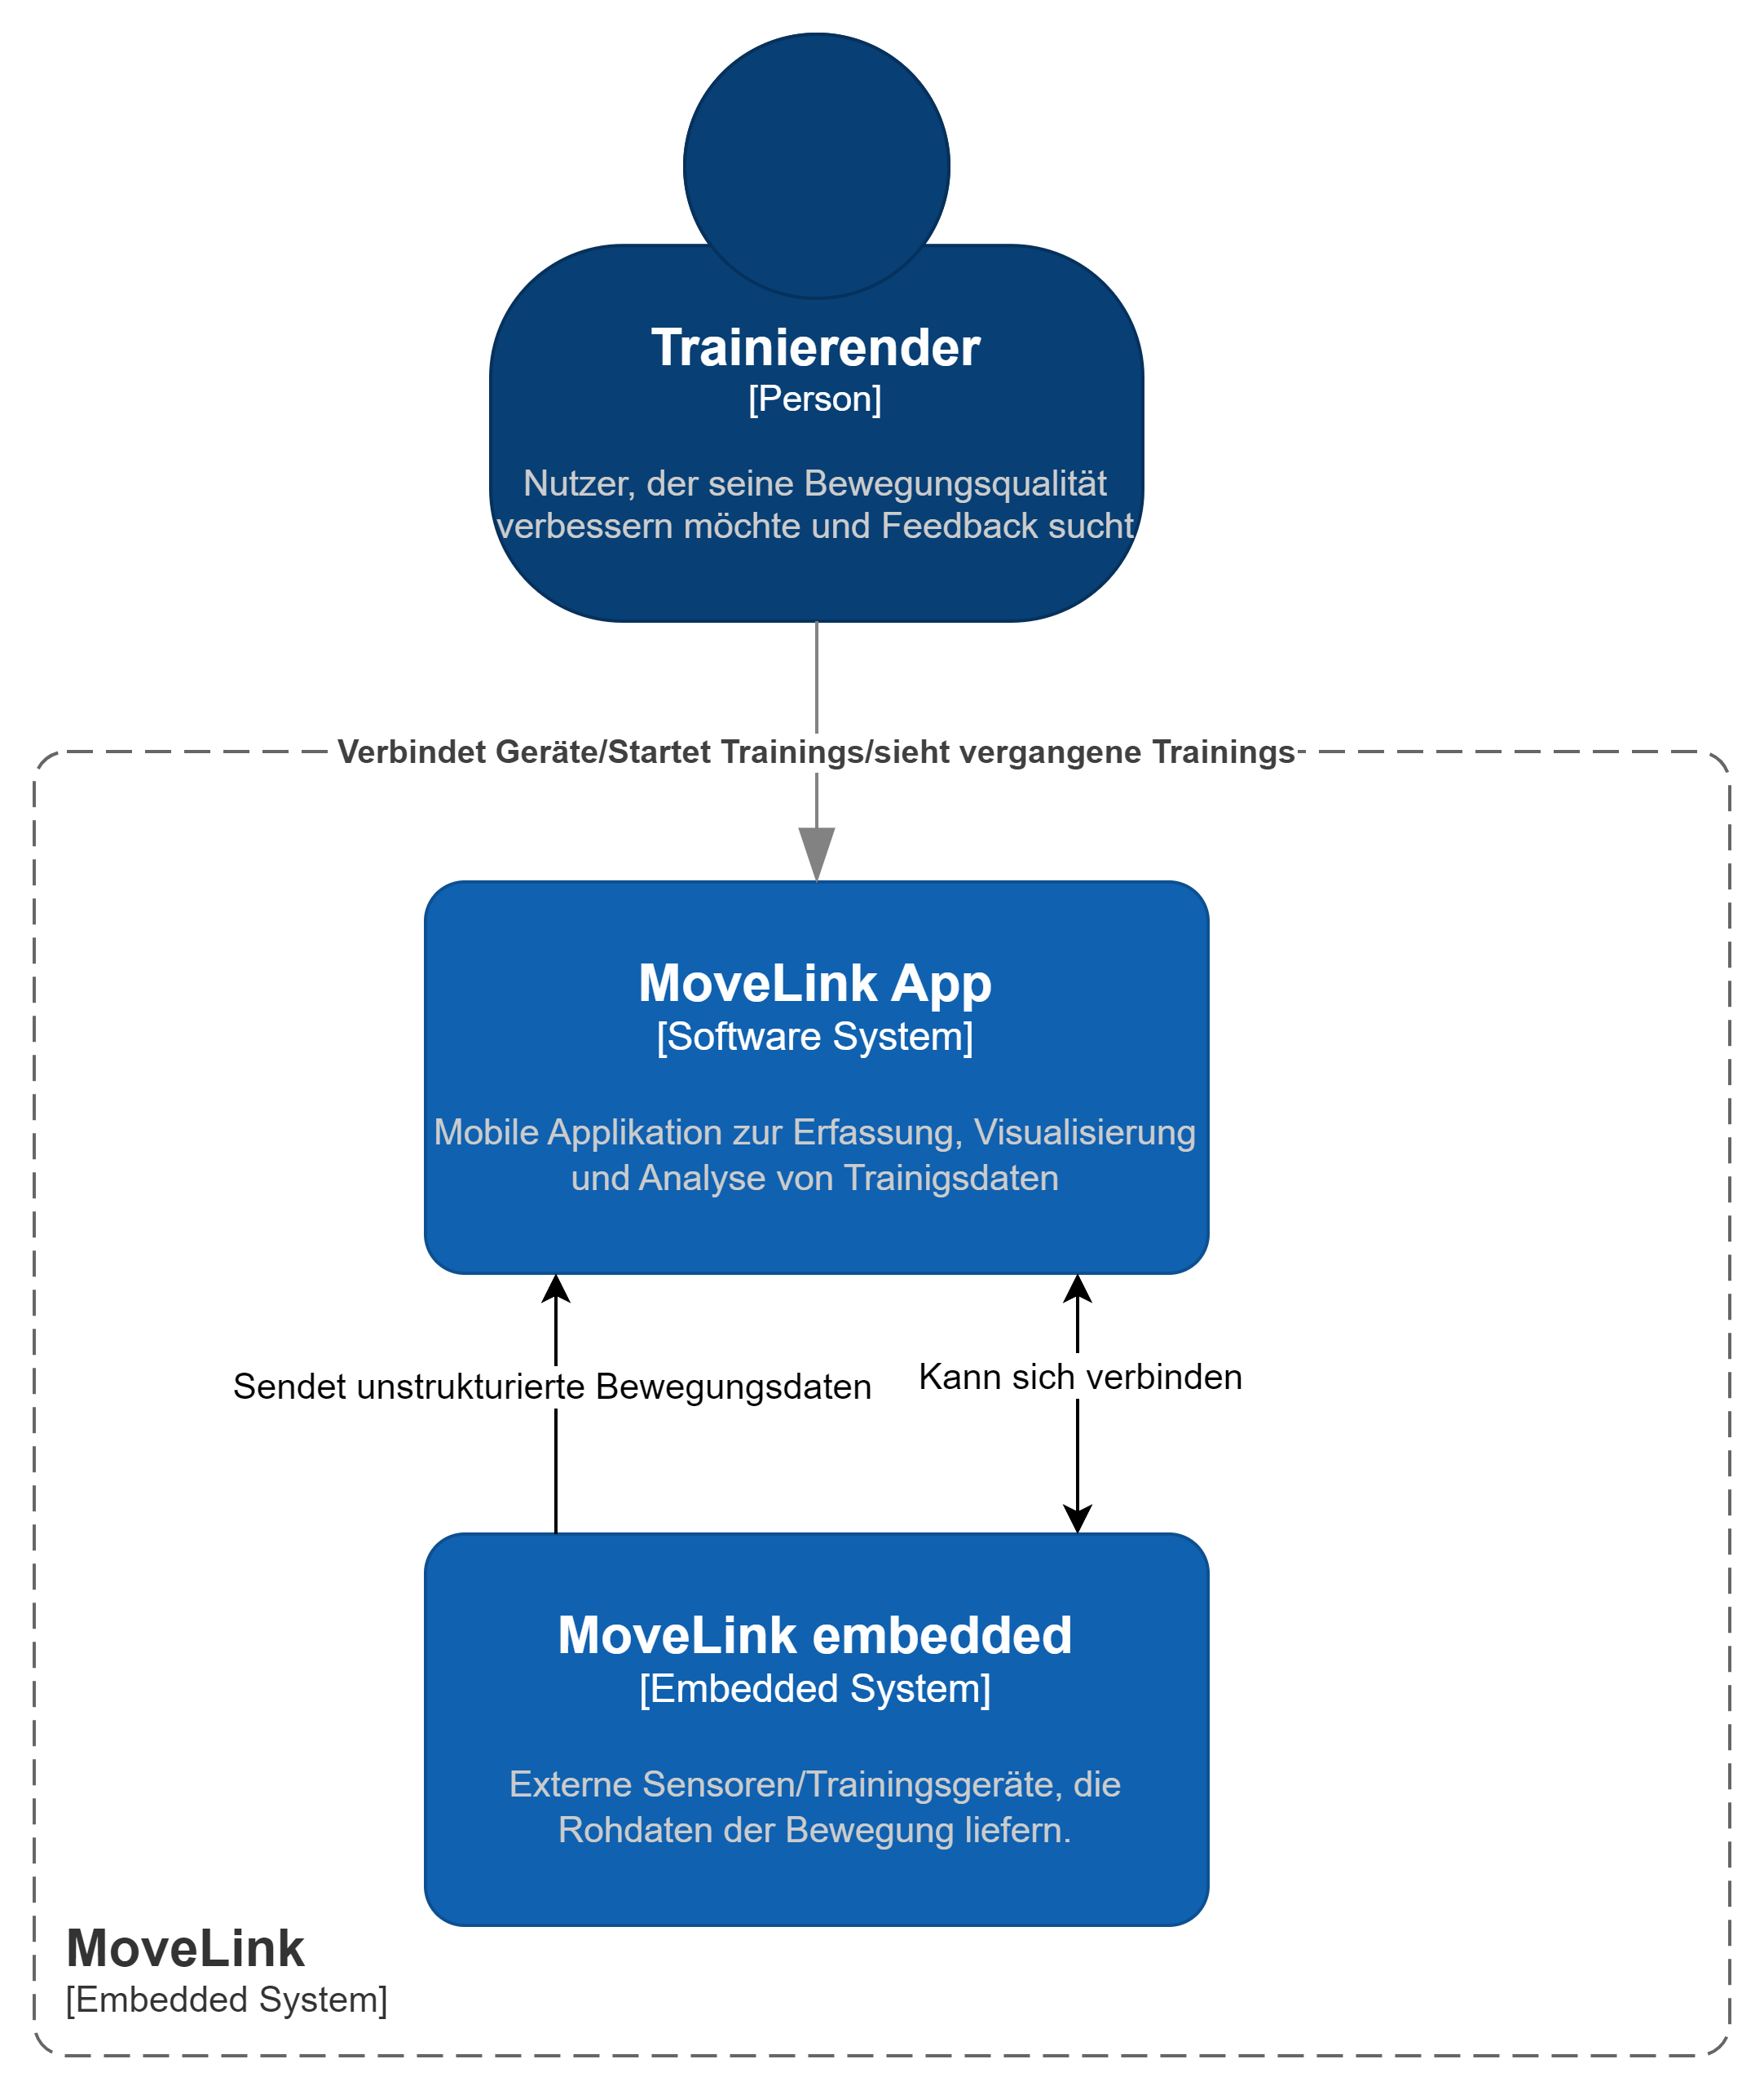
\includegraphics[width=\textwidth]{img/C4C1.png}
    \caption{System Kontext MoveLink}
    \label{fig:system_kontext}
\end{figure}

\vspace{.5cm}
\newpage
% =============================================================================
\section{Use Cases}
% =============================================================================
Bevor eine Architekturerläuterung folgt, sollen zunächst die folgenden Use Cases definiert werden. Diese dienen dem Verständnis der Anforderungen an das System. Jeder Use Case wird durch eine kurze Beschreibung und nachfolgend durch eine Auflistung der Schritte, die zur Erfüllung des Use Cases notwendig sind, definiert.

\vspace{0.5cm}
\textbf{UC-1: Trainingsger\"at verbinden} \vspace{.25cm} \newline 
\textit{Akteur:} Trainierender \quad 
\textit{Vorbedingung:} Trainingsger\"at eingeschaltet \newline
\textit{Beschreibung:} Als Trainierender m\"ochte ich mein Trainingsger\"at mit der App verbinden k\"onnen, um Trainingsdaten erfassen zu k\"onnen.
\begin{enumerate}[nosep]
    \item Eingabe: Ich als trainierender öffne die App, Ausgabe: Ich sehe eine Möglichkeit/Reiter Hardwaregeräte anzuzeigen.
    \item Eingabe: Ich als trainierender klicke auf den Reiter Hardwaregeräte, Ausgabe: Ich sehe eine Liste der verfügbaren Hardwaregeräte und mit welchen Hardwaregeräten ich verbunden bin.
    \item Eingabe: Ich als trainierender klicke auf ein Hardwaregerät in der Liste auf verbinden, Ausgabe: Ich sehe eine Detailansicht des ausgewählten Hardwaregeräts und dass dies mit der App verbunden ist.
\end{enumerate}

\vspace{0.5cm}

\textbf{UC-2: Echtzeit-Training überwachen} \vspace{.25cm} \newline 
\textit{Akteur:} Trainierender \quad 
\textit{Vorbedingung:} Trainingsgerät verbunden \newline
\textit{Beschreibung:} Ich als Trainierender möchte mein Training in Echtzeit überwachen können, um direkt Feedback zu meiner Ausführung zu erhalten.
\begin{enumerate}[nosep]
    \item Eingabe: Ich als trainierender öffne die App, Ausgabe: Ich sehe eine Möglichkeit/Reiter mein Training zu starten.
    \item Eingabe: Ich als trainierender klicke auf den Reiter "Training starten", Ausgabe: Ich sehe eine Detailansicht des ausgewählten Trainings und die Möglichkeit mein Training zu starten.
    \item Eingabe: Ich als trainierender drücke den Start Button in der Detailansicht des Trainings, Ausgabe: Die App demonstriert mir Bewegungen, welche nachzumachen sind.
    \item Eingabe: Ich als trainierender mache die Bewegung nach, Ausgabe: Die App visualisiert die Bewegung in Echtzeit und vergleicht diese mit der Demonstration. Gibt positives Feedback, wenn die Bewegung korrekt ausgeführt wurde.
\end{enumerate}

\vspace{0.5cm}

\textbf{UC-3: Trainingsdaten einsehen} \vspace{.25cm} \newline 
\textit{Akteur:} Trainierender \quad 
\textit{Vorbedingung:} Vergangene Trainingseinheit vorhanden \newline
\textit{Beschreibung:} Ich als Trainierender möchte vergangene Trainingseinheiten einsehen können, um meine Fortschritte zu verfolgen.
\begin{enumerate}[nosep]
    \item Eingabe: Ich als trainierender öffne die App, Ausgabe: Ich sehe eine Möglichkeit/Reiter vergangene Trainingseinheiten anzuzeigen.
    \item Eingabe: Ich als trainierender klicke auf den Reiter "Trainingseinheiten", Ausgabe: Ich sehe eine Liste der vergangenen Trainingseinheiten an.
    \item Eingabe: Ich wähle eine Trainingseinheit aus der Liste aus, Ausgabe: Die App zeigt die historischen Bewegungsdaten grafisch an.
\end{enumerate}

\subsubsection*{Funktionale Anforderungen} \vspace{.25cm}
\begin{itemize}[topsep=0pt, parsep=0pt, itemsep=10pt]
    \item \textbf{FA1:} Das System muss einen Reiter oder eine Navigationsm\"oglichkeit f\"ur Hardwareger\"ate / Trainings / vergangene Trainingseinheiten anzeigen. (aus UC-1, UC-2, UC-3)
    \item \textbf{FA2:} Das System muss mir eine Liste von verfügbaren Hardwareger\"ate und mit welchen Hardwareger\"aten ich verbunden bin anzeigen. (aus UC-1)
    \item \textbf{FA3:} Das System muss einen verbindungsaufbau mit dem Hardwareger\"at herstellen k\"onnen. (aus UC-1)
    \item \textbf{FA4:} Das System muss eine Detailansicht f\"ur ein ausgew\"ahltes Training anzeigen. (aus UC-2)
    \item \textbf{FA5:} Das System muss Bewegungsdatenstr\"ome empfangen und verarbeiten k\"onnen. (aus UC-2)
    \item \textbf{FA6:} Das System muss die empfangenen Bewegungen in Echtzeit visualisieren. (aus UC-2)
    \item \textbf{FA7:} Das System muss historische Bewegungsdaten grafisch anzeigen k\"onnen. (aus UC-3)
\end{itemize}

\vspace{1cm}
\subsubsection*{Nicht-funktionale Anforderungen -- Muss-Kriterien} \vspace{.25cm}
\begin{itemize}[topsep=0pt, parsep=0pt, itemsep=10pt]
    \item \textbf{NF1 -- Latenz:} Die E2E-Latenz vom Sensor bis zur Darstellung muss $\leq$ \textbf{100\,ms} sein.
    \item \textbf{NF2 -- Zuverl\"assigkeit:} Bei einem Verbindungsabbruch muss die App den Nutzer benachrichtigen und automatisch Reconnect-Versuche starten.
    \item \textbf{NF3 -- Usability:} Das Pairing darf maximal zwei Nutzerinteraktionen erfordern.
\end{itemize}

\vspace{1cm}
\subsubsection*{Rahmenbedingungen} \vspace{.25cm}
\begin{itemize}[topsep=0pt, parsep=0pt, itemsep=10pt]
    \item \textbf{R1:} Die Applikationen muss auf android devices laufen.
\end{itemize}

\newpage
% =============================================================================
\section{Systemarchitektur}
% =============================================================================

\vspace{.25cm}
%\subsection{Gew\"ahlte Architektur: Containerisierte Monolith-Architektur}
%\vspace{.25cm}
%Die Architektur konzentriert sich auf die Applikationsschicht und folgt einem dreischichtigen Container-Modell, das modular aufgebaut ist und sich optimal f\"ur ein lokales Deployment eignet:
%\vspace{-.25cm}
%\begin{figure}[H]
%    \centering
%    \resizebox{\textwidth}{!}{%
%    \begin{tikzpicture}[
%        box/.style={draw=black!70, thick, rounded corners=4pt, minimum width=3.5cm, minimum height=1.4cm, align=center},
%        arrow/.style={<->, thick, >=stealth, draw=black!80},
%        label_top/.style={font=\scriptsize, midway, above, text=black!90},
%        label_bot/.style={font=\scriptsize, midway, below, text=black!80},
%        boundary/.style={draw=black!50, dashed, rounded corners=6pt, thick}
%    ]
%        \draw[boundary, fill=black!2] (7.3, -1.5) rectangle (16.7, 1.6);
%        \node[font=\scriptsize\itshape, text=black!70, anchor=north] at (12, 1.5) {Backend-Infrastruktur (Docker-Host)};
%
%        \node[box, fill=hkared!5] (sensor) at (-3.5, 0) {
%            \textbf{Sensor} \\
%            \scriptsize XIAO nRF52840 \\
%            \scriptsize \textit{+ IMU}
%        };
%        \node[box, fill=hkared!10] (frontend) at (3.5, 0) {
%            \textbf{Mobile Client} \\
%            \scriptsize Frontend-App \\
%            \scriptsize \textit{AP 1}
%        };
%        \node[box, fill=hkared!25] (backend) at (9.5, 0) {
%            \textbf{API Gateway} \\
%            \scriptsize Backend-Container \\
%            \scriptsize \textit{AP 2}
%        };
%        \node[box, fill=hkared!40] (database) at (15, 0) {
%            \textbf{Persistenz} \\
%            \scriptsize Datenbank-Container \\
%            \scriptsize \textit{AP 3}
%        };
%
%        \draw[arrow] (sensor) --
%            node[label_top] {BLE}
%            node[label_bot] {(GATT)}
%        (frontend);
%        \draw[arrow] (frontend) --
%            node[label_top] {HTTPS / WSS}
%            node[label_bot] {(JSON)}
%        (backend);
%        \draw[arrow] (backend) --
%            node[label_top] {TCP}
%            node[label_bot] {(SQL)}
%        (database);
%    \end{tikzpicture}%
%    } \vspace{-.5cm}
%    \caption{\"Ubersicht der Systemarchitektur, Protokolle und Arbeitspakete (AP)}
%    \label{fig:architektur_container}
%\end{figure}
%\begin{itemize}[topsep=0pt, parsep=0pt, itemsep=10pt]
%    \item \textbf{Sensor (extern):} Der XIAO nRF52840 mit IMU-Sensor erfasst Bewegungsdaten und sendet sie via BLE/GATT an die App. Er ist bewusst au\ss{}erhalb des Docker-Hosts angesiedelt, da es sich um externe Hardware handelt.
%    \item \textbf{Frontend-App (AP\,1):} Stellt die Benutzeroberfl\"ache f\"ur den Trainierenden bereit und ist zust\"andig f\"ur BLE-Verbindungsmanagement sowie Echtzeit-Visualisierung.
%    \item \textbf{Backend-Container (AP\,2):} Isolierter Server als zentrales API-Gateway. Verarbeitet Echtzeit-Datenstr\"ome und bietet REST-Schnittstellen f\"ur statische Anfragen.
%    \item \textbf{Datenbank-Container (AP\,3):} Kapselt die Datenhaltung. Speichert Nutzerprofile sowie die f\"ur UC-3 ben\"otigten historischen Trainingsdaten persistent.
%\end{itemize}
%\vspace{.5cm}
%\subsection{Diskussion von Alternativen}
%\vspace{.5cm}
%F\"ur die Umsetzung des Projekts steht ein Zeitbudget von insgesamt rund 180 Stunden (ca. 60 Stunden pro Person) zur Verf\"ugung. Zur Evaluierung der optimalen Systemarchitektur wurden drei Alternativen untersucht:
%\vspace{.25cm}
%\begin{table}[H]
%\centering
%\small
%\renewcommand{\arraystretch}{1.3}
%\begin{tabularx}{\textwidth}{>{\raggedright\arraybackslash}p{4.2cm} >{\raggedright\arraybackslash}X >{\raggedright\arraybackslash}X}
%    \toprule
%    \textbf{Architekturansatz} & \textbf{Vorteile} & \textbf{Nachteile} \\
%    \midrule
%
%    \textbf{Client-Server (Microservices)} \newline
%    \scriptsize Entkoppelte Frontend-/Backend-Services
%        & \vspace{-0.3cm}\begin{itemize}[leftmargin=*, nosep]
%            \item Klare \textit{Separation of Concerns}
%            \item Unabh\"angig skalierbar
%            \item Hohe Technologie-Flexibilit\"at
%          \end{itemize}
%        & \vspace{-0.3cm}\begin{itemize}[leftmargin=*, nosep]
%            \item Hoher Infrastrukturaufwand
%            \item Netzwerklatenzen
%            \item Hohe Komplexit\"at (PoC)
%          \end{itemize} \\
%    \midrule
%
%    \textbf{Client-Server (Monolith)} \newline
%    \scriptsize Zentrale Backend-Logik
%        & \vspace{-0.3cm}\begin{itemize}[leftmargin=*, nosep]
%            \item Geringe Latenz (In-Memory)
%            \item Einfaches Deployment \& Testing
%            \item Geringer Overhead (PoC)
%          \end{itemize}
%        & \vspace{-0.3cm}\begin{itemize}[leftmargin=*, nosep]
%            \item Nur vertikale Skalierung
%            \item Starke Kopplung bei Wachstum
%            \item \textit{Single Point of Failure}
%          \end{itemize} \\
%    \midrule
%
%    \textbf{Publisher-Subscriber} \newline
%    \scriptsize Ereignisgesteuert (z.\,B. MQTT)
%        & \vspace{-0.3cm}\begin{itemize}[leftmargin=*, nosep]
%            \item Sehr gut skalierbar
%            \item Ideal f\"ur Daten-Streams (IoT)
%            \item Lose gekoppelte Kommunikation
%          \end{itemize}
%        & \vspace{-0.3cm}\begin{itemize}[leftmargin=*, nosep]
%            \item Broker erforderlich
%            \item Hoher Overhead (PoC)
%            \item Erschwertes Debugging
%          \end{itemize} \\
%    \bottomrule
%\end{tabularx}
%\caption{Vergleich der evaluierten Architekturmuster}
%\label{tab:architektur_vergleich}
%\end{table}
%
%\textbf{Begr\"undung:} \vspace{.25cm} \newline Unter Abw\"agung der Ressourcenrestriktionen (180 Stunden) erweist sich die \textbf{monolithische Client-Server-Architektur} als die zielf\"uhrendste L\"osung. Sie minimiert den Infrastruktur-Overhead, erlaubt schnelle Entwicklungszyklen und erf\"ullt die Echtzeit-Anforderungen durch direkte In-Memory-Aufrufe. Potenzielle Konflikte bei der parallelen Team-Entwicklung werden durch eine saubere interne Modulstruktur vermieden.
%\vspace{.5cm}
%% =============================================================================
%\section{Technologieauswahl}
%% =============================================================================
%\vspace{.5cm}
%Die Auswahl der Technologien orientiert sich an den Ressourcenrestriktionen (Zeiteffizienz) sowie der Notwendigkeit, die Arbeitspakete klar voneinander zu entkoppeln.
%
%\vspace{.5cm}
%\begin{table}[H]
%\centering
%\small
%\renewcommand{\arraystretch}{1.5}
%\begin{tabularx}{\textwidth}{>{\raggedright\arraybackslash}p{3cm} >{\raggedright\arraybackslash}p{4cm} >{\raggedright\arraybackslash}X}
%    \toprule
%    \textbf{Schicht} & \textbf{Technologie} & \textbf{Entscheidungsbegr\"undung} \\
%    \midrule
%
%    \textbf{Embedded} \newline (AP 3)
%        & XIAO nRF52840 \newline C/C++ (Arduino/Zephyr)
%        & Integriertes BLE; kompakter Formfaktor; stromsparend; direkte IMU-Anbindung \"uber I\textsuperscript{2}C. \\
%    \midrule
%
%    \textbf{Mobile Client} \newline (AP 1)
%        & Cross-Platform Framework \newline (React Native / Flutter)
%        & \vspace{-0.3cm}\begin{itemize}[leftmargin=*, nosep]
%            \item Single-Codebase f\"ur iOS und Android.
%            \item Etablierte BLE-Bibliotheken (GATT-Support).
%            \item Hohe Rendering-Performance f\"ur Live-Charts.
%          \end{itemize} \\
%    \midrule
%
%    \textbf{API \& Gateway} \newline (AP 2)
%        & Node.js (TypeScript) \newline oder Python (FastAPI)
%        & \vspace{-0.3cm}\begin{itemize}[leftmargin=*, nosep]
%            \item Non-Blocking I/O f\"ur parallele Live-Streams.
%            \item Native WebSocket- und REST-Unterst\"utzung.
%          \end{itemize} \\
%    \midrule
%
%    \textbf{Persistenz}
%        & PostgreSQL
%        & ACID-konforme Speicherung; JSONB-Support f\"ur schemaloser Sensordaten (Zeitreihen). \\
%    \midrule
%
%    \textbf{Echtzeit- \newline kommunikation}
%        & WebSockets (WSS)
%        & Bidirektionaler Vollduplex-Kanal; Latenz $< 100$\,ms; kein HTTP-Polling-Overhead. \\
%    \midrule
%
%    \textbf{Infrastruktur}
%        & Docker \& Docker Compose
%        & Reproduzierbarer lokaler Betrieb aller Dienste mit einem Befehl; kein Cloud-Hosting n\"otig. \\
%
%    \bottomrule
%\end{tabularx}
%\caption{\"Ubersicht und Begr\"undung des gew\"ahlten Technologie-Stacks}
%\label{tab:technologieauswahl}
%\end{table}
%
%\newpage
%% =============================================================================
%\section{Umsetzung und Implementierung}
%% =============================================================================
%\vspace{.25cm}
%\subsection{Embedded-Schicht -- XIAO nRF52840 (AP\,3)}
%\vspace{.5cm}
%\begin{placeholder}
%\textbf{\color{placeholderborder}TODO -- Wird nach Abschluss der Implementierung erg\"anzt \newline (AP\,3 -- Erlind Sejdiu)}
%
%\begin{itemize}[topsep=0pt, parsep=0pt, itemsep=5pt]
%    \item Beschreibung der Firmware-Architektur (Arduino/Zephyr RTOS)
%    \item IMU-Initialisierung und Kalibrierung (LSM6DS3TR-C \"uber I\textsuperscript{2}C)
%    \item Abtastrate und Datenformat der Sensorwerte (Accelerometer, Gyroskop)
%    \item BLE-Service-Definitionen (GATT-Service UUID, Characteristic-Layout)
%    \item Implementierung der BLE-Notifications / Advertising
%    \item Energieverwaltung und Verbindungsparameter
%    \item Code-Snippets der Kernfunktionalit\"at
%\end{itemize}
%\end{placeholder}
%\vspace{.25cm}
%\subsection{Backend -- API-Gateway und Containerisierung (AP\,2)}
%\vspace{.5cm}
%\begin{placeholder}
%\textbf{\color{placeholderborder}TODO -- Wird nach Abschluss der Implementierung erg\"anzt \newline (AP\,2 -- Luca Sch\"oneberg)}
%
%\begin{itemize}[topsep=0pt, parsep=0pt, itemsep=5pt]
%    \item Projektstruktur und gew\"ahltes Framework (Node.js/FastAPI)
%    \item REST-API-Endpunkte (Routen, Request-/Response-Schemata)
%    \item WebSocket-Handler: Verbindungsmanagement und Broadcast-Logik
%    \item Datenbankschema (Tabellen: Nutzer, Sessions, Sensorwerte)
%    \item Docker-Compose-Konfiguration (Services, Netzwerke, Volumes)
%    \item Umgebungsvariablen und Konfigurationsmanagement
%    \item Sequenzdiagramm des Datenflusses (BLE-Eingang bis WS-Ausgang)
%\end{itemize}
%\end{placeholder}
%\vspace{.25cm}
%\subsection{Frontend -- Mobile Applikation (AP\,1)}
%\vspace{.5cm}
%\begin{placeholder}
%\textbf{\color{placeholderborder}TODO -- Wird nach Abschluss der Implementierung erg\"anzt \newline (AP\,1 -- Devin Uyan)}
%
%\begin{itemize}[topsep=0pt, parsep=0pt, itemsep=5pt]
%    \item Projektstruktur und Komponentenarchitektur (z.\,B. React Native Screens)
%    \item BLE-Verbindungsmanagement: Scan, Pairing, GATT-Notification-Handling
%    \item WebSocket-Client-Implementierung und Zustandsmanagement
%    \item Echtzeit-Visualisierungskomponente (Bibliothek, Darstellungsform, Achsen)
%    \item Historien-Ansicht: Abruf und Darstellung vergangener Sessions
%    \item UI/UX-Entscheidungen (Navigation, Farbgebung, Feedbackelemente)
%    \item Screenshots / Screen-Recordings der fertigen App
%\end{itemize}
%\end{placeholder}
%
%\newpage
%% =============================================================================
%\section{Qualit\"atssicherung und Tests}
%% =============================================================================
%\vspace{.5cm}
%\begin{placeholder}
%\textbf{\color{placeholderborder}TODO -- Wird nach Abschluss der Implementierung erg\"anzt}
%
%Geplante Inhalte dieses Abschnitts:
%
%\begin{itemize}[topsep=0pt, parsep=0pt, itemsep=5pt]
%    \item \textbf{Teststrategie:} \"Ubersicht der eingesetzten Testmethoden \newline(Unit-, Integrations-, Systemtest)
%    \item \textbf{Backend-Tests:} Unit-Tests der REST-Endpunkte; \newline Integrationstests des WebSocket-Handlers
%    \item \textbf{Frontend-Tests:} Komponenten-Tests; manuelle UI-Tests auf Android und iOS
%    \item \textbf{End-to-End-Test:} Messung der tats\"achlichen End-to-End-Latenz (Sensor $\rightarrow$ App)
%    \item \textbf{Latenzauswertung:} Vergleich gemessene Latenz vs. Anforderung NF1 ($< 100$\,ms)
%    \item \textbf{Bekannte Einschr\"ankungen:} Abweichungen vom urspr\"unglichen Pflichtenheft
%\end{itemize}
%\end{placeholder}
%
%% =============================================================================
%\section{Fazit}
%% =============================================================================
%\vspace{.5cm}
%\begin{placeholder}
%\textbf{\color{placeholderborder}TODO -- Wird am Projektende verfasst}
%
%Geplante Inhalte dieses Abschnitts:
%
%\begin{itemize}[topsep=0pt, parsep=0pt, itemsep=5pt]
%    \item \textbf{Zusammenfassung:} Was wurde umgesetzt? \newline Wurden die Ziele aus Abschnitt~1.2 erreicht?
%    \item \textbf{Erf\"ullte Muss- und Kann-Kriterien:} R\"uckblick auf den Anforderungskatalog (Abschnitt~3.2)
%    \item \textbf{Erfahrungen:} Team-Reflexion zu Technologiewahl, \newline Architekturentscheidungen und Arbeitsteilung
%    \item \textbf{Ausblick:} M\"ogliche n\"achste Schritte \newline(ML-Integration, Produktivbetrieb, Multi-Sensor-Unterst\"utzung)
%\end{itemize}
%\end{placeholder}
%\vspace{.5cm}
%% =============================================================================
\section*{Literaturverzeichnis}
\addcontentsline{toc}{section}{Literaturverzeichnis}
% =============================================================================
\vspace{.5cm}
\begin{thebibliography}{9}

\bibitem{ble_spec}
Bluetooth SIG, \textit{Bluetooth Core Specification 5.4}, 2023. \\
\texttt{https://www.bluetooth.com/specifications/specs/core54-html/}

\bibitem{xiao_nrf52840}
Seeed Studio, \textit{XIAO nRF52840 (Sense) Wiki}, 2023. \\
\texttt{https://wiki.seeedstudio.com/XIAO\_BLE/}

\bibitem{lsm6ds3}
STMicroelectronics, \textit{LSM6DS3TR-C Datasheet}, 2019. \\
\texttt{https://www.st.com/en/mems-and-sensors/lsm6ds3tr-c.html}

\bibitem{websocket_rfc}
I. Fette, A. Melnikov, \textit{RFC 6455: The WebSocket Protocol}, IETF, 2011. \\
\texttt{https://datatracker.ietf.org/doc/html/rfc6455}

\bibitem{docker_compose}
Docker Inc., \textit{Docker Compose Documentation}, 2024. \\
\texttt{https://docs.docker.com/compose/}

\end{thebibliography}
\end{document}